\chapter{Image Warping, Inverse Mapping, and Bilinear Interpolation}
\label{ch:lesson09}

Chapter~\ref{ch:lesson08} built transformation matrices; this chapter is about actually \emph{applying} one to resample an image. The naive way to do this --- push every source pixel to its transformed location --- turns out to be broken. We see why, fix it with \textbf{inverse mapping}, and then deal with the fact that inverse mapping lands on fractional pixel coordinates that need to be \emph{interpolated}. Figure~\ref{fig:l09-1} shows the test image used throughout.

\begin{figure}[h]
\centering
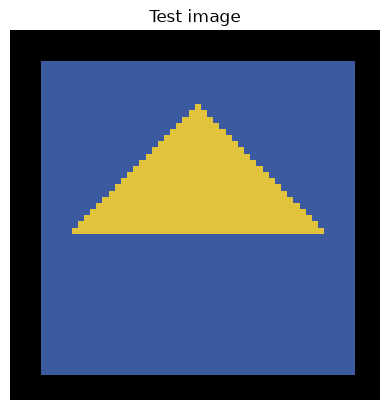
\includegraphics[width=0.3\textwidth]{figures/lesson09_fig01.png}
\caption{The test image used throughout this chapter.}
\label{fig:l09-1}
\end{figure}

\section{The problem with forward mapping}

The obvious way to warp an image: for every source pixel $(x,y)$, compute its destination $(x',y')=M(x,y)$ and copy the pixel value there. This is called \textbf{forward mapping}. It has a fundamental flaw: whereas the source pixels form a \emph{complete} grid, their transformed locations generally do not. When a transform enlarges the image (or rotates it, which locally stretches the grid along the diagonal), the destination locations spread out and leave gaps --- no source pixel happens to land exactly on some destination pixels.

\begin{lstlisting}
dst_pts = M @ src_pts
dxi, dyi = np.round(dst_pts[0]).astype(int), np.round(dst_pts[1]).astype(int)
valid = (dxi >= 0) & (dxi < w) & (dyi >= 0) & (dyi < h)
forward[dyi[valid], dxi[valid]] = img[ys.ravel()[valid], xs.ravel()[valid]]
\end{lstlisting}

For a $25^\circ$ rotation combined with a $1.6\times$ scale, only $1408$ of $3600$ destination pixels ($39\%$) receive a value, leaving visible holes (Figure~\ref{fig:l09-2}).

\begin{figure}[h]
\centering
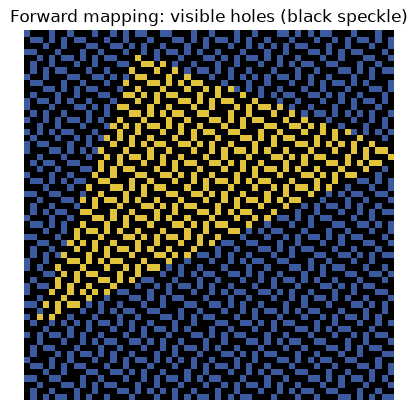
\includegraphics[width=0.3\textwidth]{figures/lesson09_fig02.png}
\caption{Forward mapping: visible holes (black speckles) where no source pixel happened to land.}
\label{fig:l09-2}
\end{figure}

\section{The fix: inverse mapping}

Instead of asking ``where does each source pixel go?'', ask the opposite question for every \emph{destination} pixel: ``where in the source image did this come from?'' That means applying the \textbf{inverse} transform $M^{-1}$ to each destination coordinate. Since we now iterate over a complete destination grid, every output pixel is guaranteed to get a value --- no holes, by construction. The catch: $M^{-1}(x',y')$ almost never lands exactly on an integer source coordinate, so a value must be \emph{interpolated} from the surrounding source pixels.

\begin{lstlisting}
M_inv = cv2.invertAffineTransform(M)
src_coords = M_inv @ dst_grid   # fractional source coordinates for every destination pixel
\end{lstlisting}

\subsection*{Nearest-neighbor interpolation}

The simplest option: round to the nearest integer source pixel. This has no holes, but is blocky --- many destination pixels round to the \emph{same} source pixel, so the image looks pixelated wherever the transform enlarges it (Figure~\ref{fig:l09-3}).

\begin{figure}[h]
\centering
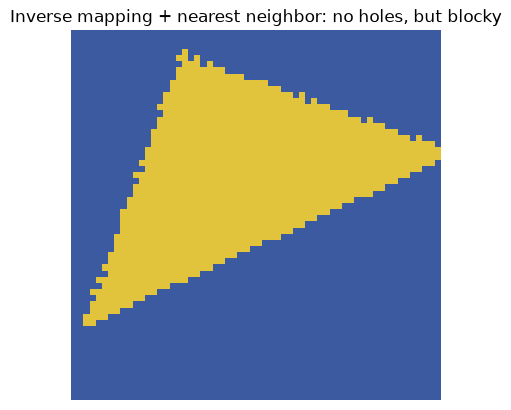
\includegraphics[width=0.3\textwidth]{figures/lesson09_fig03.png}
\caption{Inverse mapping with nearest-neighbor sampling: no holes, but blocky.}
\label{fig:l09-3}
\end{figure}

\subsection*{Bilinear interpolation}

Instead of snapping to the single nearest pixel, \textbf{bilinear interpolation} blends the 4 neighboring pixels, weighted by how close it is to each one. Let $(x_0,y_0)$ be the integer pixel just below-left of $(x,y)$, and $d_x=x-x_0$, $d_y=y-y_0$, with $0\le d_x,d_y<1$. Then
\begin{equation}
I(x,y) \approx (1{-}d_x)(1{-}d_y)\,I(x_0,y_0) + d_x(1{-}d_y)\,I(x_1,y_0) + (1{-}d_x)\,d_y\,I(x_0,y_1) + d_x\,d_y\,I(x_1,y_1),
\end{equation}
where $x_1=x_0+1$, $y_1=y_0+1$. This is just two 1D linear interpolations (along $x$, then along $y$) composed --- hence \emph{bi}linear.

\begin{lstlisting}
Ia, Ib, Ic, Id = image[y0,x0], image[y0,x1], image[y1,x0], image[y1,x1]
out = (1-dx)*(1-dy)*Ia + dx*(1-dy)*Ib + (1-dx)*dy*Ic + dx*dy*Id
\end{lstlisting}

Figure~\ref{fig:l09-4} compares the two interpolation methods.

\begin{figure}[h]
\centering
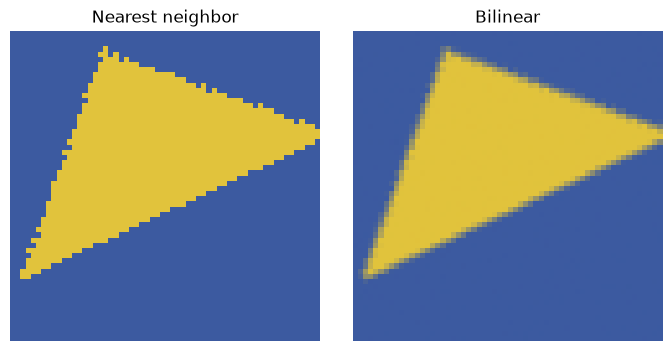
\includegraphics[width=0.55\textwidth]{figures/lesson09_fig04.png}
\caption{Nearest-neighbor (left) vs.\ bilinear (right). Bilinear has smooth edges around the triangle and rectangle instead of jagged steps --- the classic trade-off is a softer, slightly blurrier image in exchange for removing aliasing artifacts.}
\label{fig:l09-4}
\end{figure}

\subsection*{Sanity check against OpenCV}

\code{cv2.warpAffine} does exactly this --- inverse mapping plus interpolation --- internally, agreeing closely with the from-scratch version (Figure~\ref{fig:l09-5}).

\begin{figure}[h]
\centering
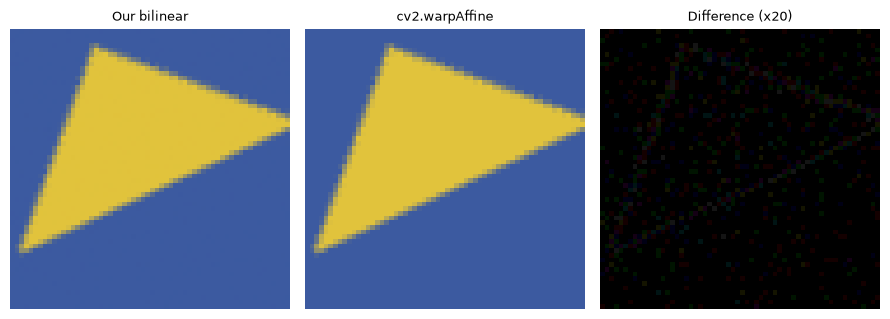
\includegraphics[width=0.85\textwidth]{figures/lesson09_fig05.png}
\caption{Our bilinear implementation vs.\ \code{cv2.warpAffine(..., flags=cv2.INTER\_LINEAR)}: max pixel difference is $1$ (out of 255), mean difference $0.092$. The tiny remaining gap comes from OpenCV using fixed-point rounding internally for speed rather than full floating-point arithmetic.}
\label{fig:l09-5}
\end{figure}

\subsection*{Exercises}
\begin{enumerate}
  \item Why doesn't the forward-mapping holes problem happen when the transform only \emph{shrinks} the image? Try a scale of \code{0.5} instead of \code{1.6} in the forward-mapping example and see what fraction of destination pixels get filled.
  \item Extend \code{bilinear\_sample} to bicubic interpolation conceptually: instead of a $2\times2$ neighborhood, what neighborhood size would you need, and what property would you want the weights to satisfy at the sample points?
  \item Time \code{bilinear\_sample} against \code{cv2.warpAffine} on a larger image (e.g.\ $800\times800$) using \code{\%timeit}. By how much faster is the OpenCV version, and why?
\end{enumerate}

\vfill
\fullcode{lesson09}{lesson09_warping_interpolation}
